\documentclass[12pt]{article}

\usepackage{indentfirst} % Adds identation to first paragraph in sections

% Language setting
\usepackage[english]{babel}

% Set page size and margins
\usepackage[letterpaper,top=2cm,bottom=2cm,left=3cm,right=3cm,marginparwidth=1.75cm]{geometry}

% Set double spacing across document
\usepackage{setspace}
\doublespacing

% Useful packages
\usepackage{amsfonts}
\usepackage{amsmath}
\usepackage{graphicx}
\usepackage[colorlinks=true, allcolors=blue]{hyperref}
\usepackage{float} 
\usepackage{titling}
\usepackage{caption} % allows centering captions with \captionsetup

\title{Performance Comparison of MobileOne and FastViT with Traditional CNN and ViT Architectures for Image Classification Tasks in Mobile Deployments}
\author{Adarley Luiz Grando Filho}
\date{December 18, 2024}

\begin{document}

% Capa
\begin{center}
{\LARGE
École de Technologie Supérieure}

Department of Systems Engineering

SYS843 - Réseaux de neurones et systèmes flous

Final Project Report
\end{center}

\vspace*{\fill}

\begin{center}
    \singlespacing \Large \textbf{\\\thetitle \\}
\end{center}

\begin{center}
	\vspace{1cm}
	\normalsize	
	Professor \\
	\large
	\textbf{Eric Granger}
	
	\vspace{1cm}
	\normalsize	
	Author \\
	\large
	\textbf{\theauthor}
\end{center}

\vspace*{\fill}

\begin{center}
    \textbf{Montréal\\
    \thedate}
\end{center}

\thispagestyle{empty} % Retira o cabeçalho e o rodapé da página

\newpage



\tableofcontents
\newpage

\section{Introduction}

\subsection{Domain of application}
Real-time image classification tasks on mobile devices have wide-ranging applications, from on-device photo organization and augmented reality experiences to embedded systems for drones, robotics, and surveillance. The ability to classify images efficiently on mobile hardware—without relying on cloud processing—can reduce latency, improve user privacy, and lower communication costs. Such capabilities are increasingly important in healthcare (mobile diagnostic tools), retail (product recognition), and navigation (visual-based assistance).

\subsection{Problematic}
While traditional architectures such as convolutional neural networks (CNNs) and vision transformers (ViTs) achieve state-of-the-art accuracy in image classification, they often require substantial computational resources. Deploying these models directly onto mobile devices can lead to high latency, increased memory usage, and energy constraints. Although specialized mobile-friendly architectures like MobileOne and FastViT have emerged to address these issues, it remains challenging to compare these diverse architectures under a common experimental setup. Understanding their trade-offs in accuracy, latency, and resource usage is crucial for selecting the best model in real-world deployments.

\subsection{Objectives of the project}
This project aims to:
\begin{itemize}
    \item Compare the performance of four neural network architectures (ResNet, TinyViT, MobileOne, and FastViT) in mobile deployment scenarios.
    \item Evaluate trade-offs in accuracy and latency-related metrics when running these models on-device.
    \item Investigate the benefits of fine-tuning FastViT from ImageNet-1k pretrained weights versus training from scratch.
    \item Provide practical insights for practitioners looking to choose a suitable architecture for real-time, on-device image classification tasks.
\end{itemize}

\subsection{Structure of the document}
The document is structured as follows:
\begin{enumerate}
    \item \textbf{Introduction:} Presents the domain, the key issues, and the objectives of the project.
    \item \textbf{Summary of the techniques studied:} Provides a general overview of the algorithms (CNNs, ViTs, MobileOne, and FastViT), including an expanded algorithmic description.
    \item \textbf{Experimental methodology:} Details the experimental protocols, training configurations, model deployments, and the chosen performance metrics.
    \item \textbf{Simulation results:} (Skeleton) Will present the measured results, comparisons, and analyses.
    \item \textbf{Conclusion:} (Skeleton) Will summarize the findings and provide recommendations.
\end{enumerate}

\section{Summary of the techniques studied}

\subsection{General block diagram of the system}
Figure~\ref{fig:block_diagram} presents a general block diagram of the image classification system. An input image is passed through a chosen neural network model, which produces a probability distribution over the class labels. A decision layer selects the highest-probability class as the prediction.

In this project Convolutional Neural Networks and Vision Transformers are the neural networks being studied. Figure~\ref{fig:cnn_diagram} illustrates a general diagram of a Convolutional Neural Network architecture. Figure~\ref{fig:vision_transformer_architecture} illustrates a general diagram of a Vision Transformer architecture.

\begin{figure}[]
\centering
\captionsetup{justification=centering,margin=1cm}
\setlength{\unitlength}{0.9pt}
\begin{picture}(475,120)

% Input Image
\put(10,50){\framebox(80,40){\parbox{70pt}{\centering Input Image}}}

% Arrow from Input to Preprocessing
\put(90,70){\vector(1,0){40}}

% Preprocessing (optional block)
% If you do not have preprocessing steps, skip this part and connect input directly to model
\put(130,50){\framebox(80,40){\parbox{70pt}{\centering Preprocessing}}}
\put(210,70){\vector(1,0){40}}

% Neural Network Model (ResNet / TinyViT / MobileOne / FastViT)
\put(250,30){\framebox(100,80){\parbox{90pt}{\centering Chosen Neural\\ Network Model}}}

% Arrow from Model to Output
\put(350,70){\vector(1,0){40}}

% Output Class Prediction
\put(390,50){\framebox(80,40){\parbox{70pt}{\centering Class Prediction}}}

\end{picture}
\caption{General block diagram of the mobile image classification system.}
\label{fig:block_diagram}
\end{figure}

\begin{figure}[]
    \centering
    \captionsetup{justification=centering,margin=1cm}
    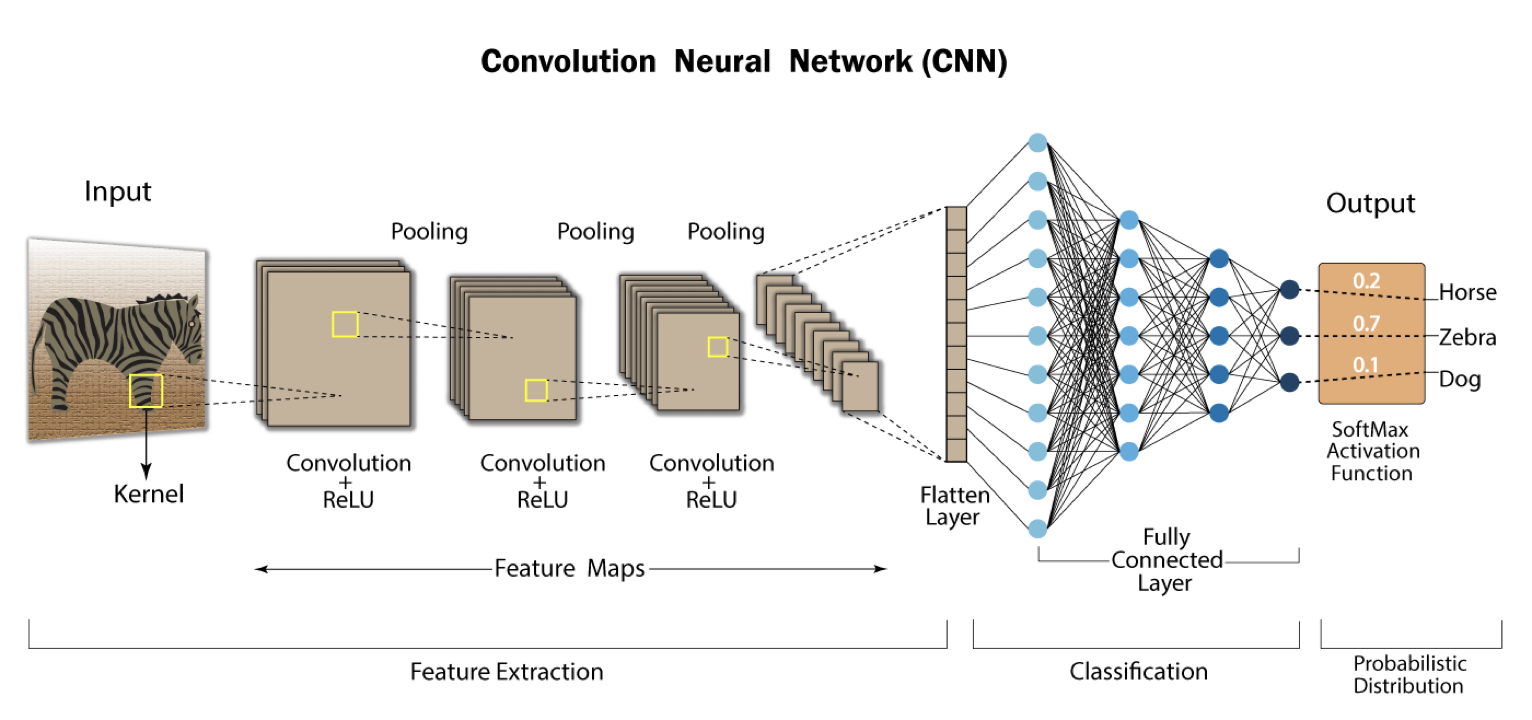
\includegraphics[width=0.85\linewidth]{cnn_diagram.png}
    \caption{\label{fig:cnn_diagram}Convolutional Neural Network general architecture (Abdullah, 2022 \cite{cnn_diagram}).}
\end{figure}

\begin{figure}[]
    \centering
    \captionsetup{justification=centering,margin=1cm}
    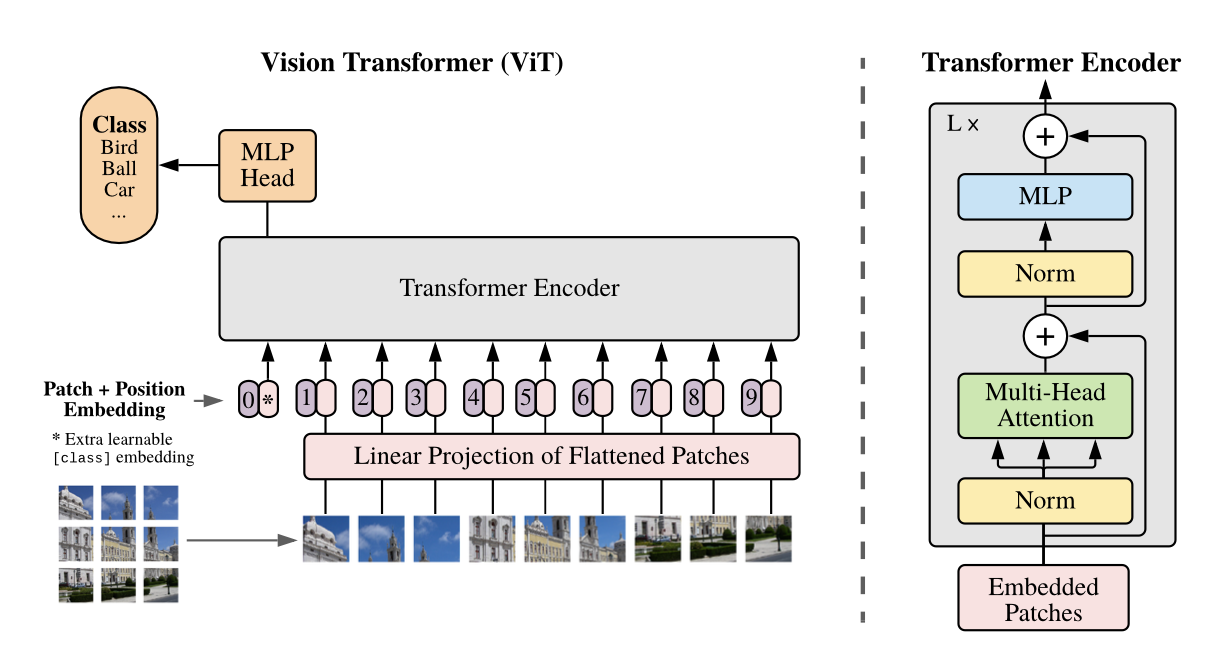
\includegraphics[width=0.75\linewidth]{vision_transformer_architecture.png}
    \caption{\label{fig:vision_transformer_architecture}Vision Transformer general architecture (Dosovitskiy, 2021 \cite{dosovitskiy2021imageworth16x16words}).}
\end{figure}

\subsection{Algorithmic description of the studied techniques}

In this project, four architectures are considered: a traditional CNN (ResNet), a traditional vision transformer (TinyViT), a mobile-optimized CNN (MobileOne), and a mobile-optimized hybrid vision transformer (FastViT).

\subsubsection*{Convolutional Neural Networks (CNNs) - ResNet}
Convolutional Neural Networks use convolution filters to extract spatial hierarchies of features from images. As data flows through successive convolutional layers, the network identifies increasingly complex features—edges and corners in early layers, and objects or concepts in deeper layers. Pooling layers reduce spatial dimensions, and fully connected layers map extracted features to class probabilities.

\textbf{ResNet} \cite{he2015deepresiduallearningimage} introduces residual learning to address the training difficulties of very deep networks. It incorporates shortcut (skip) connections that bypass certain layers, allowing gradients to flow more easily through the network. Figure \ref{fig:resnet_residual_learning} illustrates this connection. Mathematically, if a set of layers is designed to approximate a function $F(x)$, ResNet reformulates this into learning $F(x) + x$, where $x$ is the input. This design mitigates the vanishing gradients problem and enables training of extremely deep models without a drop in accuracy. ResNet models are well-known benchmarks in vision tasks, providing a strong baseline for accuracy.

\begin{figure}[]
    \centering
    \captionsetup{justification=centering,margin=1cm}
    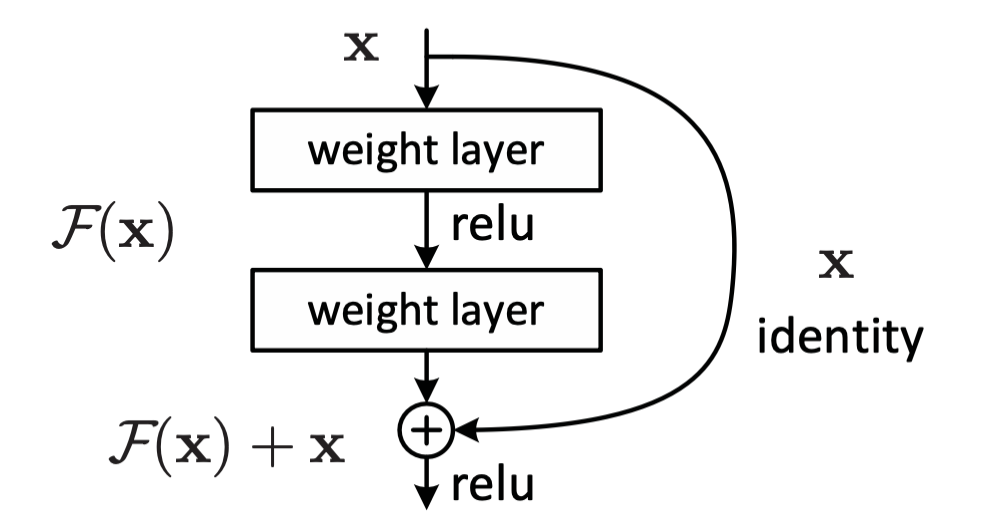
\includegraphics[width=0.5\linewidth]{resnet_residual_learning.png}
    \caption{\label{fig:resnet_residual_learning}Residual learning employed with a shortcut connection between layers in a ResNet (He, 2015 \cite{he2015deepresiduallearningimage}).}
\end{figure}

\subsubsection*{Vision Transformers (ViTs) - TinyViT}
\textbf{Vision Transformers} \cite{dosovitskiy2021imageworth16x16words} adapt the transformer architecture \cite{vaswani2023attentionneed}, originally developed for NLP, to image classification. Instead of feeding sequences of words, ViTs split the input image into fixed-size patches. Each patch is flattened and linearly projected into an embedding. The transformer encoder, composed of multi-head self-attention and feed-forward layers, models relationships between patches, capturing global context.

Key aspects of ViTs:
\begin{itemize}
    \item \textit{Patch Embeddings:} Images are divided into non-overlapping patches. Each patch acts like a ``token'', analogous to words in a sentence.
    \item \textit{Positional Encodings:} Added to patch embeddings to retain spatial order.
    \item \textit{Self-Attention:} Allows each patch to attend to all others, capturing global dependencies. This can lead to high accuracy, especially when large datasets are used.
\end{itemize}

Vision Transformers (ViTs), while excellent at capturing global context and delivering high accuracy, are generally too large in parameter count and computational demands to be deployed efficiently on mobile hardware. Their massive size often leads to prohibitively high memory usage and inference times, making them impractical for real-time, on-device applications. To address this issue and still represent the capabilities of transformer-based architectures in our comparisons, a more compact variant known as TinyViT was chosen. By drastically reducing the scale of the model, TinyViT maintains many of the transformer’s advantages while remaining small enough to feasibly run on a smartphone or similarly constrained device. This approach allows a fair performance comparison of a transformer-based solution without dismissing them due to their high resource demands.

\subsubsection*{MobileOne: A Mobile-Optimized CNN}
\textbf{MobileOne} \cite{vasu2023mobileoneimprovedmillisecondmobile} is a convolutional architecture specifically designed for efficient inference on mobile devices. It employs several strategies:
\begin{itemize}
    \item \textit{Depthwise Separable Convolutions:} Factorize a standard convolution into a depthwise and a pointwise convolution, drastically reducing computations \cite{howard2017mobilenetsefficientconvolutionalneural}.
    \item \textit{Structural Reparameterization:} During training, overparameterized branches (like parallel convolutions) help the model learn rich representations. At inference, these branches are ``merged'' into a single convolution, reducing model complexity and latency.
    \item \textit{Simplicity at Inference:} Unlike ResNet, which maintains skip connections, MobileOne’s inference architecture is streamlined, minimizing memory reads/writes and synchronization overhead.
\end{itemize}
The result is a model that can match or exceed the accuracy of classical CNNs like ResNet but is significantly faster and lighter on mobile hardware.

\subsubsection*{FastViT: A Mobile-Optimized Hybrid Vision Transformer}
\textbf{FastViT} \cite{vasu2023fastvitfasthybridvision} combines elements of ViTs and CNNs to reduce latency on mobile devices:
\begin{itemize}
    \item \textit{Hybrid Architecture:} In early layers, FastViT replaces computationally expensive self-attention with large kernel convolutions that capture extensive receptive fields without the heavy complexity of global attention.
    \item \textit{RepMixer Blocks:} Inspired by MobileOne, FastViT uses reparameterizable token-mixing blocks that employ depthwise convolutions and skip connections during training. At inference time, these blocks simplify into a latency-efficient form.
    \item \textit{Train-Time Overparameterization, Inference-Time Streamlining:} Similar to MobileOne, FastViT is more complex during training but prunes unnecessary complexity at inference.
\end{itemize}
The result is a model that retains much of the ViT’s accuracy and global context modeling but is faster and more resource-friendly on mobile devices.

\section{Experimental methodology}

\subsection{Dataset description}

\subsubsection{CIFAR-10}
CIFAR-10 is a commonly used benchmark dataset for image classification. It consists of 60,000 color images of size 32x32 pixels, organized into 10 classes (e.g., airplane, car, bird, cat). The dataset is well-known, allowing for straightforward comparisons with previous works. Despite being smaller and simpler than datasets like ImageNet, CIFAR-10 still provides a suitable environment for testing model training in small setups like it is the case for this project.

\subsubsection{ImageNet-1k}
ImageNet-1k is a large-scale image classification dataset widely used as a standard benchmark in computer vision. It consists of 1,000 classes and over one million images, with high visual complexity and diversity. Pre-training models on ImageNet-1k often leads to improved generalization and transferability to other tasks and datasets. In this project, ImageNet-1k-pretrained weights are referenced to compare how initial training on a large and more complex dataset affects performance on smaller datasets like CIFAR-10.

\subsection{Protocol to train FastViT}

The model FastViT-T8 was selected for experimentation with training. Being the smallest version of FastViT with only 4.05 million parameters, this model allowed optimizing its hyperparameters, and multiple training processes to be experimented in a timely manner.

The following subsections describe the detailed protocol adopted for training and evaluating the accuracy of FastViT on the CIFAR-10 dataset. This protocol was used to train the model from scratch, and also to fine-tune a pretrained version of the model with ImageNet-1k weights.

\subsubsection{Dataset Splitting}
The CIFAR-10 dataset, consisting of 60,000 images across 10 classes, was divided into three splits:
\begin{itemize}
    \item \textbf{Training Set:} 40,000 images selected from the original 50,000 training samples.
    \item \textbf{Validation Set:} 10,000 images held out from the training set to guide hyperparameter selection and prevent overfitting.
    \item \textbf{Test Set:} The standard 10,000 images reserved for final accuracy evaluation.
\end{itemize}
This partitioning strategy ensures a dedicated validation split for hyperparameter tuning and an untouched test set for final performance assessment.

\subsubsection{Hyperparameter Optimization}
Before conducting full-length training runs, a dedicated hyperparameter search process was carried out to identify optimal configurations for the model. The optimization was performed with a custom made script to test possible values using the Optima library \cite{optima}, which specializes in handling linear and non-linear constrained optimization problems. The approach was as follows:

\begin{enumerate}
    \item \textbf{Script Implementation:} A custom script was developed to systematically test different combinations of hyperparameters for a given model.
    \item \textbf{Short Training Runs:} For each combination of hyperparameters, a short training process of 10 epochs was executed using the validation set. These short runs allowed rapid experimentation across a wide range of configurations within a practical timeframe.
    \item \textbf{Selection Criterion:} Each short run’s performance was evaluated based on the loss achieved after 10 epochs. The combination that yielded the lowest loss was considered the optimal hyperparameter set for that particular model.
\end{enumerate}

The hyperparameters tested various batch sizes, learning rates, weight decays, optimizers, and learning rate schedulers:
\begin{itemize}
  \item \textbf{Batch Sizes:} 32, 64, 128, or 256
  \item \textbf{Learning Rates:} Ranging from $1^{-5}$ to $1^{-2}$
  \item \textbf{Weight Decays:} Ranging from $1^{-4}$ to $1^{-1}$
  \item \textbf{Optimizers:} Stochastic Gradient Descent (SGD), Adam, or AdamW
  \item \textbf{LR Schedulers:} StepLR (decaying every step), ReduceLROnPlateau, or \\ CosineAnnealingLR
\end{itemize}

The range of values selected to perform the tests were inspired from hyperparameters that the researchers who developed FastViT used and documented in its original paper. The exact hyperparameter values from the paper could not be used because they would require a computer with high performance to allow training. Specially the batch size of 1024 documented in FastViT original paper requires a lot of RAM to perform the gradient calculations, since this amount of images would have to be loaded to memory at once. A Google Colab PRO subscription allowed testing with bigger batch sizes of up to 256.

In total, the script evaluated 50 distinct hyperparameter combinations. By selecting the configuration yielding the best validation performance, the process ensured that full training runs started from a well-tuned configuration.

\subsubsection{Training Strategies}
Once the optimal hyperparameters were identified, FastViT was trained from scratch using the 40,000 training images and validated against the 10,000 validation images. In addition to training FastViT from scratch, an alternative strategy was employed: fine-tuning from a version pretrained on ImageNet-1k. This approach explored whether large-scale pretraining could enhance accuracy or generalization for the smaller CIFAR-10 dataset.

\subsubsection{Accuracy Evaluation}
After the full training was completed and the final model parameters were selected, FastViT’s accuracy was evaluated on the standardized CIFAR-10 test set containing 10,000 images. This test split remained untouched during training and hyperparameter tuning, ensuring an unbiased estimate of generalization capability.

\subsection{Protocol to evaluate performance}

The evaluation protocol was designed to assess how various neural network architectures—both traditional and mobile-optimized—perform on a mobile device. The models selected represent a range of parameter counts and architectural complexities, enabling meaningful comparisons. Smaller variants highlight efficiency and speed, while larger models demonstrate the upper bounds of accuracy and resource usage. By comparing both extremes, we gain a clearer understanding of trade-offs between model size, accuracy, and latency on constrained mobile hardware.

Table \ref{tab:model_param_counts} lists the models under consideration, spanning different families (ResNet, TinyViT, MobileOne, and FastViT) and parameter scales. Among these, FastViT-SA12, MobileOne-S3, TinyViT-11M, and ResNet-18 form a group with similar parameter counts, making them ideal for direct comparisons. Likewise, examining variants like FastViT-T8 or MobileOne-S1 (smaller) against heavier counterparts like TinyViT-21M or ResNet-34 (larger) can provide insights into how scaling up model size affects latency and other performance metrics.

\begin{table}[]
    \centering
    \doublespacing
    \captionsetup{justification=centering,margin=1cm}
    \begin{tabular}{l|c}
        \hline
        \textbf{Model} & \textbf{Parameter Count (M)} \\
        \hline
        FastViT-T8 & 4.05 \\
        FastViT-SA12 & 11.6 \\
        MobileOne-S1 & 4.89 \\
        MobileOne-S3 & 10.3 \\
        TinyViT-11M & 11 \\
        TinyViT-21M & 21.2 \\
        ResNet-18 & 11.7 \\
        ResNet-34 & 21.8 \\
        \hline
    \end{tabular}
    \caption{Models evaluated along with their parameter counts.}
    \label{tab:model_param_counts}
\end{table}

The subsequent subsections detail the procedures for on-device deployment and measurement collection. Latency-related metrics (such as compute units, prediction median, load median, and compilation median) were recorded on an iPhone 13 Pro to reflect realistic mobile inference conditions. By correlating these measurements with model complexity and accuracy, the evaluation aims to guide practitioners in selecting architectures best suited to their specific deployment scenarios.

\subsubsection{On-Device Deployment}
Pretrained models were converted into a mobile-compatible format using Core ML Tools \cite{coremltools}, and then deployed on an iPhone 13 Pro using Xcode \cite{xcode}. This deployment stage allowed for assessing model responsiveness, compatibility, and practical suitability for real-time applications directly on mobile hardware.

\subsubsection{Performance Report}
To create a performance report, the model deployed on the device goes through several iterations of compile, load, and predictions. Once those are complete, the metrics are calculated by Xcode. The report shows how many operations were executed to perform a prediction, as well as which compute units—CPU, GPU, or Neural Engine—were used. It also shows statistics about the run, like median prediction time, median load time, and median compilation time.

The report also provides in-depth information about the layers of the model, like the type of operations performed, and the compute unit they ran on. Core ML optimizes each operation to run in the best compute unit available but it is possible to tweak and change this behavior if the operation is compatible with other compute units.

\subsubsection{Latency-Related Measurements}
To gauge on-device performance, latency-related metrics were collected from the deployed models. These included:
\begin{itemize}
    \item \textbf{Compute Units:} Indicating the level of computational resources the device allocated for the model’s inference.
    \item \textbf{Prediction Median:} The median time taken to process a single image and produce a classification result.
    \item \textbf{Load Median:} The median time required to load the model into memory on the device.
    \item \textbf{Compilation Median:} The median time spent on any initial compilation or optimization steps performed by the device’s machine learning runtime before running inference.
\end{itemize}

Together, these latency-related metrics provide a practical understanding of each model’s runtime efficiency, user experience implications, and suitability for real-time mobile applications.

\subsection{Performance measures}
The key metrics used in this work are:
\begin{itemize}
    \item \textbf{Accuracy:} The proportion of correct top-1 predictions on the CIFAR-10 image test set for the trained FastViT model, and reported proportion of correct top-1 predictions on the ImageNet-1k image test set for all models.
    \item \textbf{Compute Units:} A measure related to the on-device computational resources allocated for inference.
    \item \textbf{Prediction Median:} The median time for a prediction run, reflecting how quickly a model can respond.
    \item \textbf{Load Median:} The median time taken to load the model onto the device before inference.
    \item \textbf{Compilation Median:} The median time required for any on-device model compilation or optimization steps before load.
\end{itemize}

\section{Results}
In this section the following results obtained from the experiments are documented:
\begin{itemize}
    \item \textbf{Training FastViT:} Detailed information about the training process of FastViT on CIFAR-10 (both from-scratch and fine-tuned from ImageNet-1k),
    \item \textbf{Accuracy Comparison:} Comparison of accuracy across ResNet, TinyViT, MobileOne, and FastViT on ImageNet-1k (both for smaller and bigger versions of models).
    \item \textbf{Latency-Related Measurements:} Comparison of compute units, prediction median, load median, and compilation median across all models (both for smaller and bigger versions of models).
\end{itemize}

\subsection{Training FastViT}

The following subsections describe in detail the processes of training FastViT-T8 from scratch and from pretrained weights on ImageNet-1k. Even though this model is small in parameter count, it was not feasible to successfully train it in a regular computer with limited hardware. Upon further reading of the original paper that introduced this model, it became clear that usual batch sizes of 16 or 32 would not be a good fit to train this model. The original paper suggests that a batch size of 1024 would yield better results.

In order to experiment with this model, a Google Colab Pro subscription was made, that allowed me to access a high RAM server and with better GPUs than my local machine. The high performance server allowed experimenting with bigger batch sizes of up to 256.

\subsubsection{Hyperparameter Tuning}

After running the hyperparameter tuning process with 50 different combinations, the optimal hyperparameters found for FastViT-T8 were recorded and used for the full trainings. Surprisingly, the hyperparameters used when training FastViT from scratch did not yield good results when performing full training on a pretrained version of FastViT with ImageNet-1k weights, as detailed in Section \ref{sec:training_fastvit}.

Upon further investigation, another process of hyperparameter tuning was ran with 50 different combinations of possible values, but this time a pretrained version of the model was used. The optimal hyperparameters for the pretrained version of the model with ImageNet-1k weights showed that a lower learning rate was preferred for this case. All hyperparameter values are documented in Table \ref{tab:hyperparameters}.

\begin{table}[]
    \centering
    \doublespacing
    \captionsetup{justification=centering,margin=1cm}
    \begin{tabular}{l|c|c}
        \hline
        \textbf{Parameter} & \textbf{From 0} & \textbf{Fine-tune} \\
        \hline
        Batch size & 256 & 256 \\
        \hline
        Learning rate & $1^{-3}$ & $1^{-4}$ \\
        \hline
        Weight decay & $5^{-2}$ & $5^{-2}$ \\
        \hline
        Optimizer & AdamW & AdamW \\
        \hline
        Learning rate scheduler & CosineAnnealingLR & CosineAnnealingLR \\
        \hline
    \end{tabular}
    \caption{Optimal hyperparameters found after running 50 combinations of possible values per training type of FastViT-T8.}
    \label{tab:hyperparameters}
\end{table}

\subsubsection{Training} \label{sec:training_fastvit}

When training FastViT from scratch using the hyperparameters previously identified as optimal, both training and validation loss curves improved steadily and predictably. The model converged smoothly, and over time the validation loss closely followed the training loss, indicating that the chosen learning rate and optimization parameters were well-suited for a model initialized with random weights. Figure~\ref{fig:fastvit_train_0} shows these stable, gradually declining loss curves, exemplifying a straightforward convergence pattern. In the last epochs we can see that the model continued to lower its train loss, but the validation loss stopped decreasing, indicating that the model had began to memorize the train data split, so the training needed to be halted at that point to prevent overfitting.

\begin{figure}[]
    \centering
    \captionsetup{justification=centering,margin=1cm}
    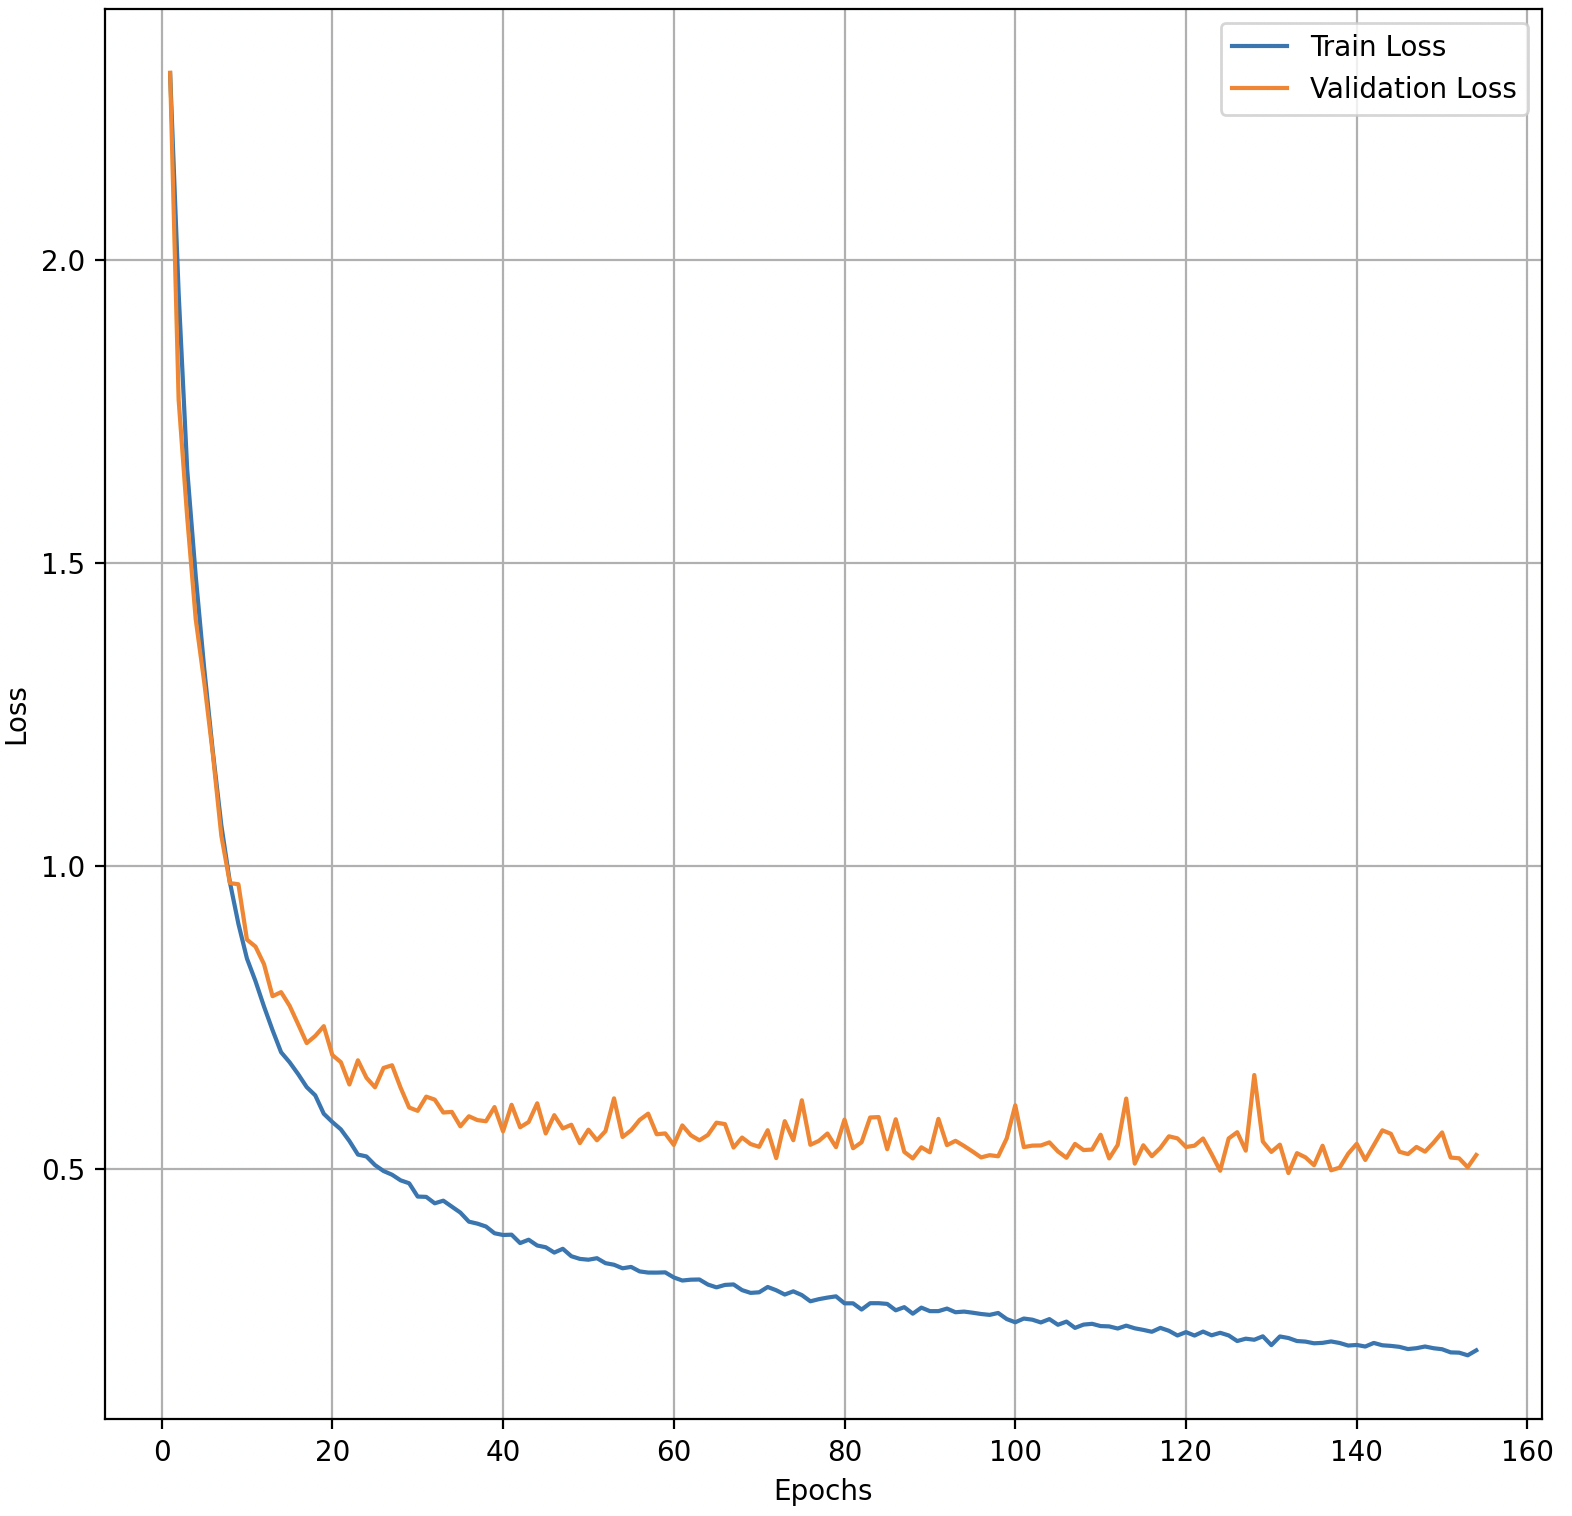
\includegraphics[width=0.6\linewidth]{fastvit_train_0.png}
    \caption{\label{fig:fastvit_train_0}Train and validation loss over training epochs of FastViT-T8 (trained from 0 on CIFAR-10).}
\end{figure}

In contrast, applying the same hyperparameters directly to a pretrained FastViT model resulted in significantly different behavior. While the training loss still trended downward, the validation loss began to oscillate after a few epochs, never settling into a stable improvement phase. This instability suggested that the learning rate and other settings optimal for from-scratch training were too aggressive for fine-tuning. As shown in Figure~\ref{fig:fastvit_train_pretrained_bad_lr}, the validation loss curve reflects a noisy and inconsistent trajectory, highlighting the need for adjusted hyperparameters when starting from pretrained weights.

\begin{figure}[]
    \centering
    \captionsetup{justification=centering,margin=1cm}
    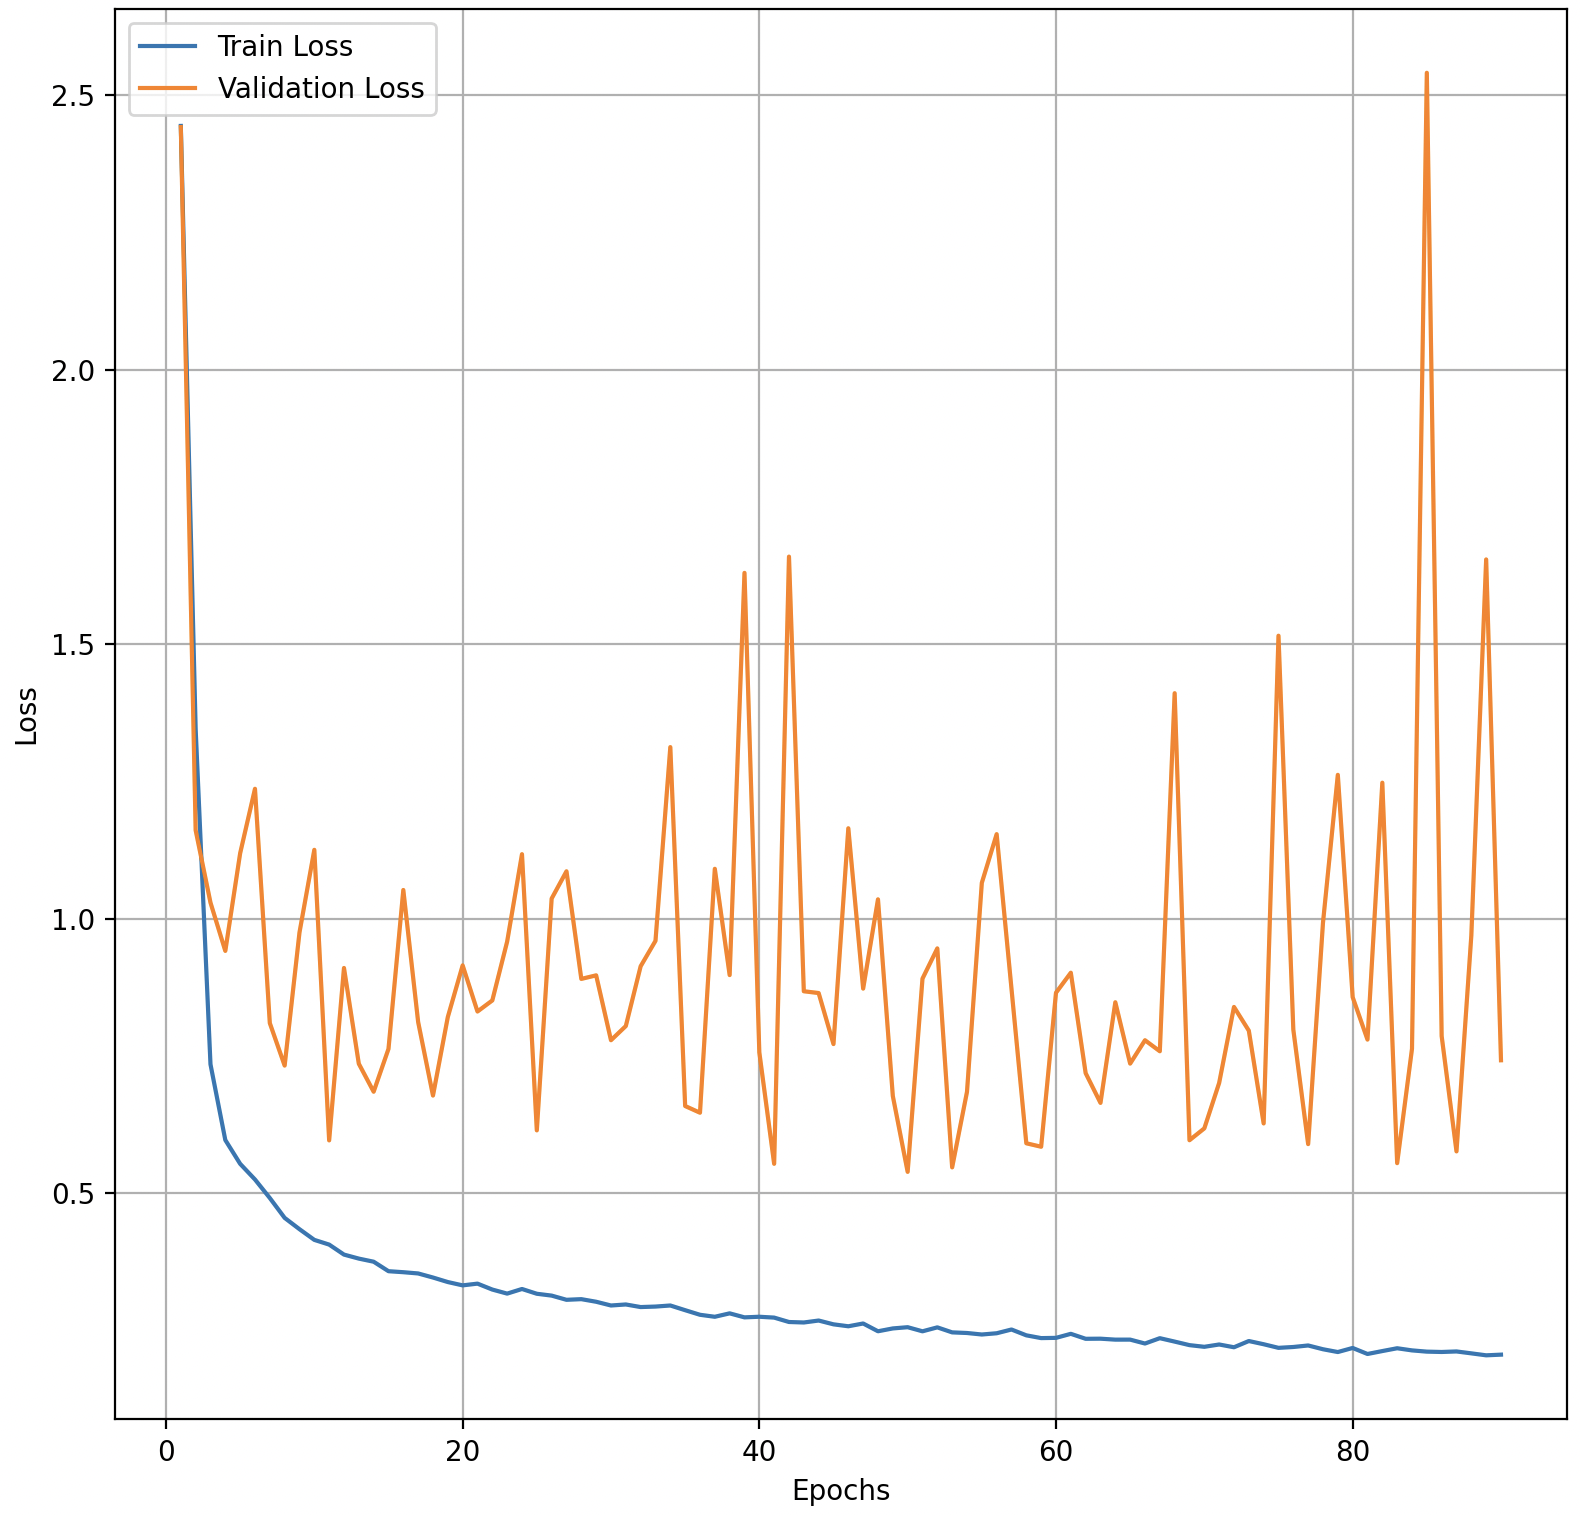
\includegraphics[width=0.6\linewidth]{fastvit_train_pretrained_bad_lr.png}
    \caption{\label{fig:fastvit_train_pretrained_bad_lr}Train and validation loss over training epochs of FastViT-T8 with bad hyperparameters for fine-tuning (fine-tuned on CIFAR-10 from pretrained weights on ImageNet-1k).}
\end{figure}

After recognizing this issue, a new round of hyperparameter optimization was conducted, this time specifically targeting the pretrained scenario. Among the 50 combinations tested, those featuring a reduced learning rate yielded more stable and consistent validation performance. Figure~\ref{fig:fastvit_train_pretrained_good_lr} shows the improved loss curves after incorporating these changes: the validation loss stabilized without the previous large oscillations. Moreover, this carefully tuned configuration not only avoided instability but also achieved better generalization than the from-scratch training, demonstrating the benefits of fine-tuning with appropriately chosen hyperparameters. 

\begin{figure}[]
    \centering
    \captionsetup{justification=centering,margin=1cm}
    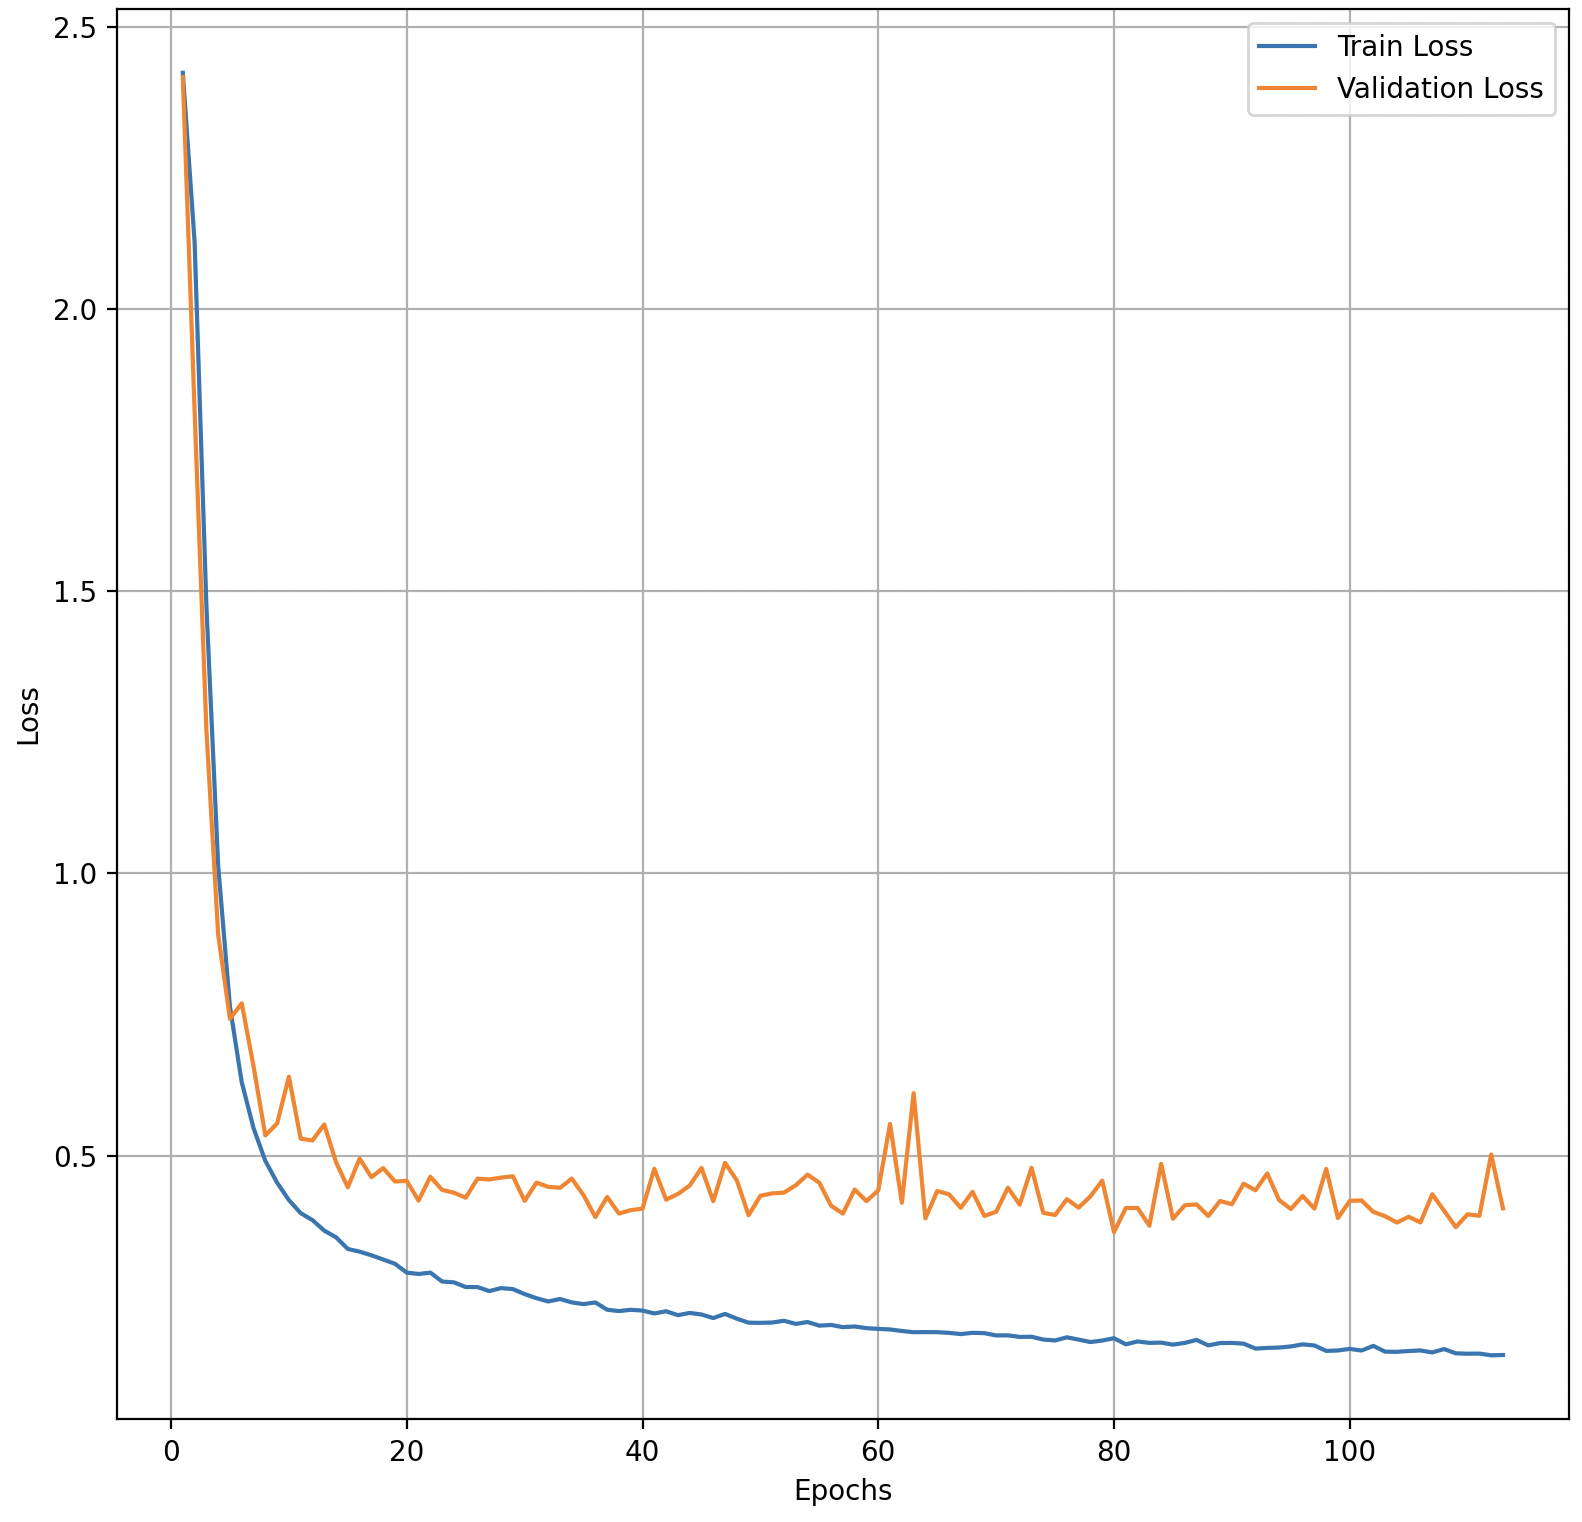
\includegraphics[width=0.6\linewidth]{fastvit_train_pretrained_good_lr.png}
    \caption{\label{fig:fastvit_train_pretrained_good_lr}Train and validation loss over training epochs of FastViT-T8 with optimized hyperparameters for fine-tuning (fine-tuned on CIFAR-10 from pretrained weights on ImageNet-1k).}
\end{figure}

\subsubsection{Accuracy on CIFAR-10}

The final top-1 accuracy in the test split of the model was of 85.28\%, when trained from scratch on CIFAR-10. The final top-1 accuracy in the test split of the model was of 88.66\%, when fine-tuned on CIFAR-10 from pretrained weights on ImageNet-1k. A confusion matrix of the most successful training process was also calculated and is illustrated in Figure~\ref{fig:fastvit_train_pretrained_cm}.

\begin{figure}[]
    \centering
    \captionsetup{justification=centering,margin=1cm}
    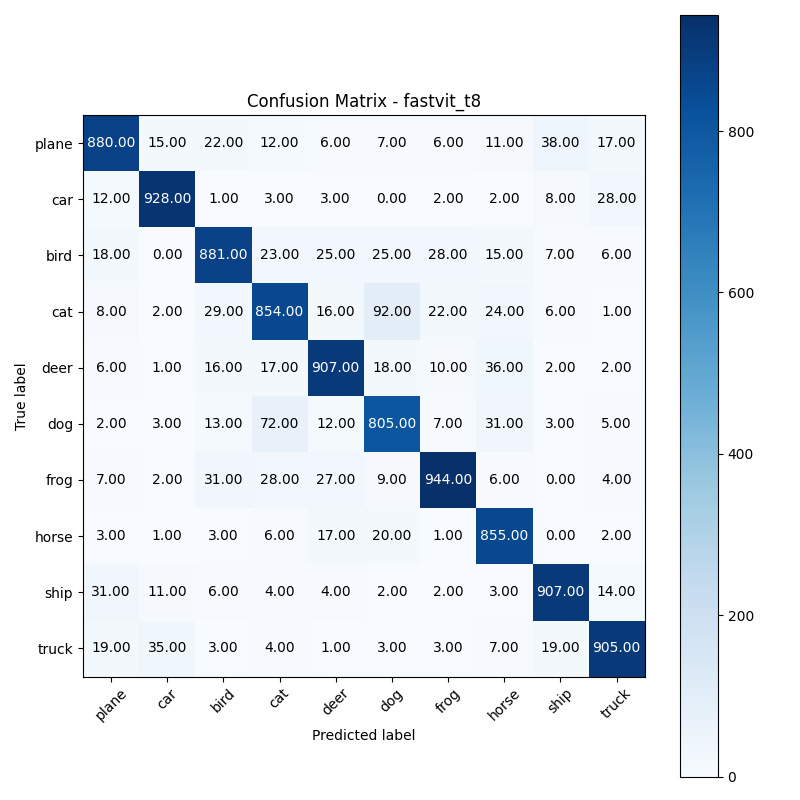
\includegraphics[width=0.75\linewidth]{fastvit_train_pretrained_cm.png}
    \caption{\label{fig:fastvit_train_pretrained_cm}Confusion Matrix after end of training of FastViT-T8 with optimized hyperparameters for fine-tuning (fine-tuned on CIFAR-10 from pretrained weights on ImageNet-1k).}
\end{figure}

\subsection{Accuracy comparison}
% Ref: https://github.com/huggingface/pytorch-image-models/blob/main/results/results-imagenet.csv
This subsection will detail top-1 accuracy on ImageNet-1k for each model. The accuracy values presented in Table \ref{tab:model_param_counts} are drawn from the Hugging Face PyTorch Image Models (timm) benchmarks \cite{pytorch-image-models}, which provide a standardized comparison of a wide range of architectures evaluated under consistent conditions on the ImageNet-1k dataset. These reported top-1 accuracy scores allow us to compare the baseline performance of the studied models before considering their latency and resource usage in mobile deployments.

\begin{table}[]
    \centering
    \doublespacing
    \captionsetup{justification=centering,margin=1cm}
    \begin{tabular}{l|c}
        \hline
        \textbf{Model} & \textbf{Top-1 accuracy (\%)} \\
        \hline
        FastViT-T8 & 76.18 \\
        FastViT-SA12 & 80.84 \\
        MobileOne-S1 & 75.77 \\
        MobileOne-S3 & 78.00 \\
        TinyViT-11M & 81.54 \\
        TinyViT-21M & 83.27 \\
        ResNet-18 & 71.49 \\
        ResNet-34 & 76.41 \\
        \hline
    \end{tabular}
    \caption{Top-1 accuracy of studied models when trained on ImageNet-1k dataset.}
    \label{tab:model_param_counts}
\end{table}

Looking at the results, we see that TinyViT models achieve the highest accuracies among the considered architectures, with TinyViT-21M reaching 83.27\% and TinyViT-11M at 81.54\%. FastViT-SA12 follows closely at 80.84\%, outperforming both MobileOne and ResNet variants. In contrast, the ResNet-18 and ResNet-34 models—representative of a more traditional CNN architecture—display lower top-1 accuracies at 71.49\% and 76.41\%, respectively. While these accuracies provide an initial ranking of models by predictive power on ImageNet-1k, the subsequent analyses will consider whether these accuracy advantages translate efficiently to on-device scenarios, where latency, memory consumption, and overall mobile performance may shift the balance of which model is most suitable.

\subsection{Latency and load comparison}
This subsection will compare the prediction median, load median, and compilation median times across the four models, providing insights into which architectures are most suitable for real-time mobile inference. Table \ref{tab:on_device_performance} illustrates these latency indicators for each model. A prediction time of around 20 ms tells that a model could support about 50 frames per second, if it were to be deployed for real time predictions.

\begin{table}[]
    \centering
    \doublespacing
    \captionsetup{justification=centering,margin=1cm}
    \begin{tabular}{l|c|c|c}
        \hline
        \textbf{Model} & \textbf{Prediction (ms)} & \textbf{Load (ms)} & \textbf{Compile (ms)} \\ \hline
        FastViT-T8 & 1.16 & 25.27 & 106.94 \\
        FastViT-SA12 & 2.34 & 28.09 & 116.76 \\
        MobileOne-S1 & 1.51 & 25.30 & 109.66 \\
        MobileOne-S3 & 2.08 & 25.54 & 104.48 \\
        TinyViT-11M & 3.37 & 25.28 & 105.75 \\
        TinyViT-21M & 4.33 & 25.59 & 118.75 \\
        ResNet-18 & 1.37 & 12.98 & 54.03 \\
        ResNet-34 & 1.94 & 15.67 & 67.52 \\
        \hline
    \end{tabular}
    \caption{On-device inference performance metrics for various models, including median prediction, load, and compile times.}
    \label{tab:on_device_performance}
\end{table}

Additionally, a comparison of the model size and the total operations to perform an inference task is provided. Table \ref{tab:model_params_ops} illustrates the total number of operations allocated to perform a single task. They represent ``computational units'' or ``workloads'' that the model’s execution engine schedules on different compute unit processors.

\begin{table}[]
    \centering
    \doublespacing
    \captionsetup{justification=centering,margin=1cm}
    \begin{tabular}{l|c|c}
        \hline
        \textbf{Model} & \textbf{Parameter Count (M)} & \textbf{Operations} \\ \hline
        FastViT-T8 & 4.05 & 191 \\
        FastViT-SA12 & 11.6 & 245 \\
        MobileOne-S1 & 4.89 & 206 \\
        MobileOne-S3 & 10.3 & 206 \\
        TinyViT-11M & 11 & 335 \\
        TinyViT-21M & 21.2 & 335 \\
        ResNet-18 & 11.7 & 54 \\
        ResNet-34 & 21.8 & 94 \\
        \hline
    \end{tabular}
    \caption{Model parameter counts and total operations measured on-device.}
    \label{tab:model_params_ops}
\end{table}

\subsection{Discussion of results}
This subsection will discuss the observed trade-offs, relating accuracy to latency-related measurements, and highlight the effects of training from scratch versus fine-tuning for FastViT.

\subsubsection{Model comparisons}
The results highlight the complex trade-offs between accuracy, latency, and model complexity in the context of mobile deployments. Models like TinyViT-21M, which exhibited some of the highest top-1 accuracy scores on ImageNet-1k, demonstrated slower on-device prediction times and a greater number of operations. Although its superior accuracy makes it an attractive choice for scenarios where predictive quality is crucial, the additional computational overhead may pose challenges for real-time, resource-constrained applications.

On the other hand, more lightweight architectures such as FastViT-T8 and MobileOne-S1 managed to offer rapid prediction times with fewer operations, making them appealing candidates for latency-sensitive use cases like real-time video processing or embedded systems. While these models may not achieve the top-tier accuracy of heavier architectures, their speed and efficiency can be critical for maintaining a responsive user experience on mobile devices. Interestingly, parameters and operations alone were not always reliable predictors of latency—some models with fewer parameters still took relatively longer to load or compile, suggesting that memory access patterns, the choice of activation functions, or hardware-level optimizations can significantly influence actual runtime performance.

Figure~\ref{fig:comparison_latency_inference} further illustrates the complexity of predicting on-device latency from model size alone. In this scatter plot, models with fewer parameters do not consistently yield lower prediction times, and conversely, some architectures with higher parameter counts achieve relatively low latency. This lack of correlation suggests that other factors—such as operator types, memory access patterns, and hardware-level optimizations—play a more decisive role in determining actual inference speed than mere parameter count.

\begin{figure}[]
    \centering
    \captionsetup{justification=centering,margin=1cm}
    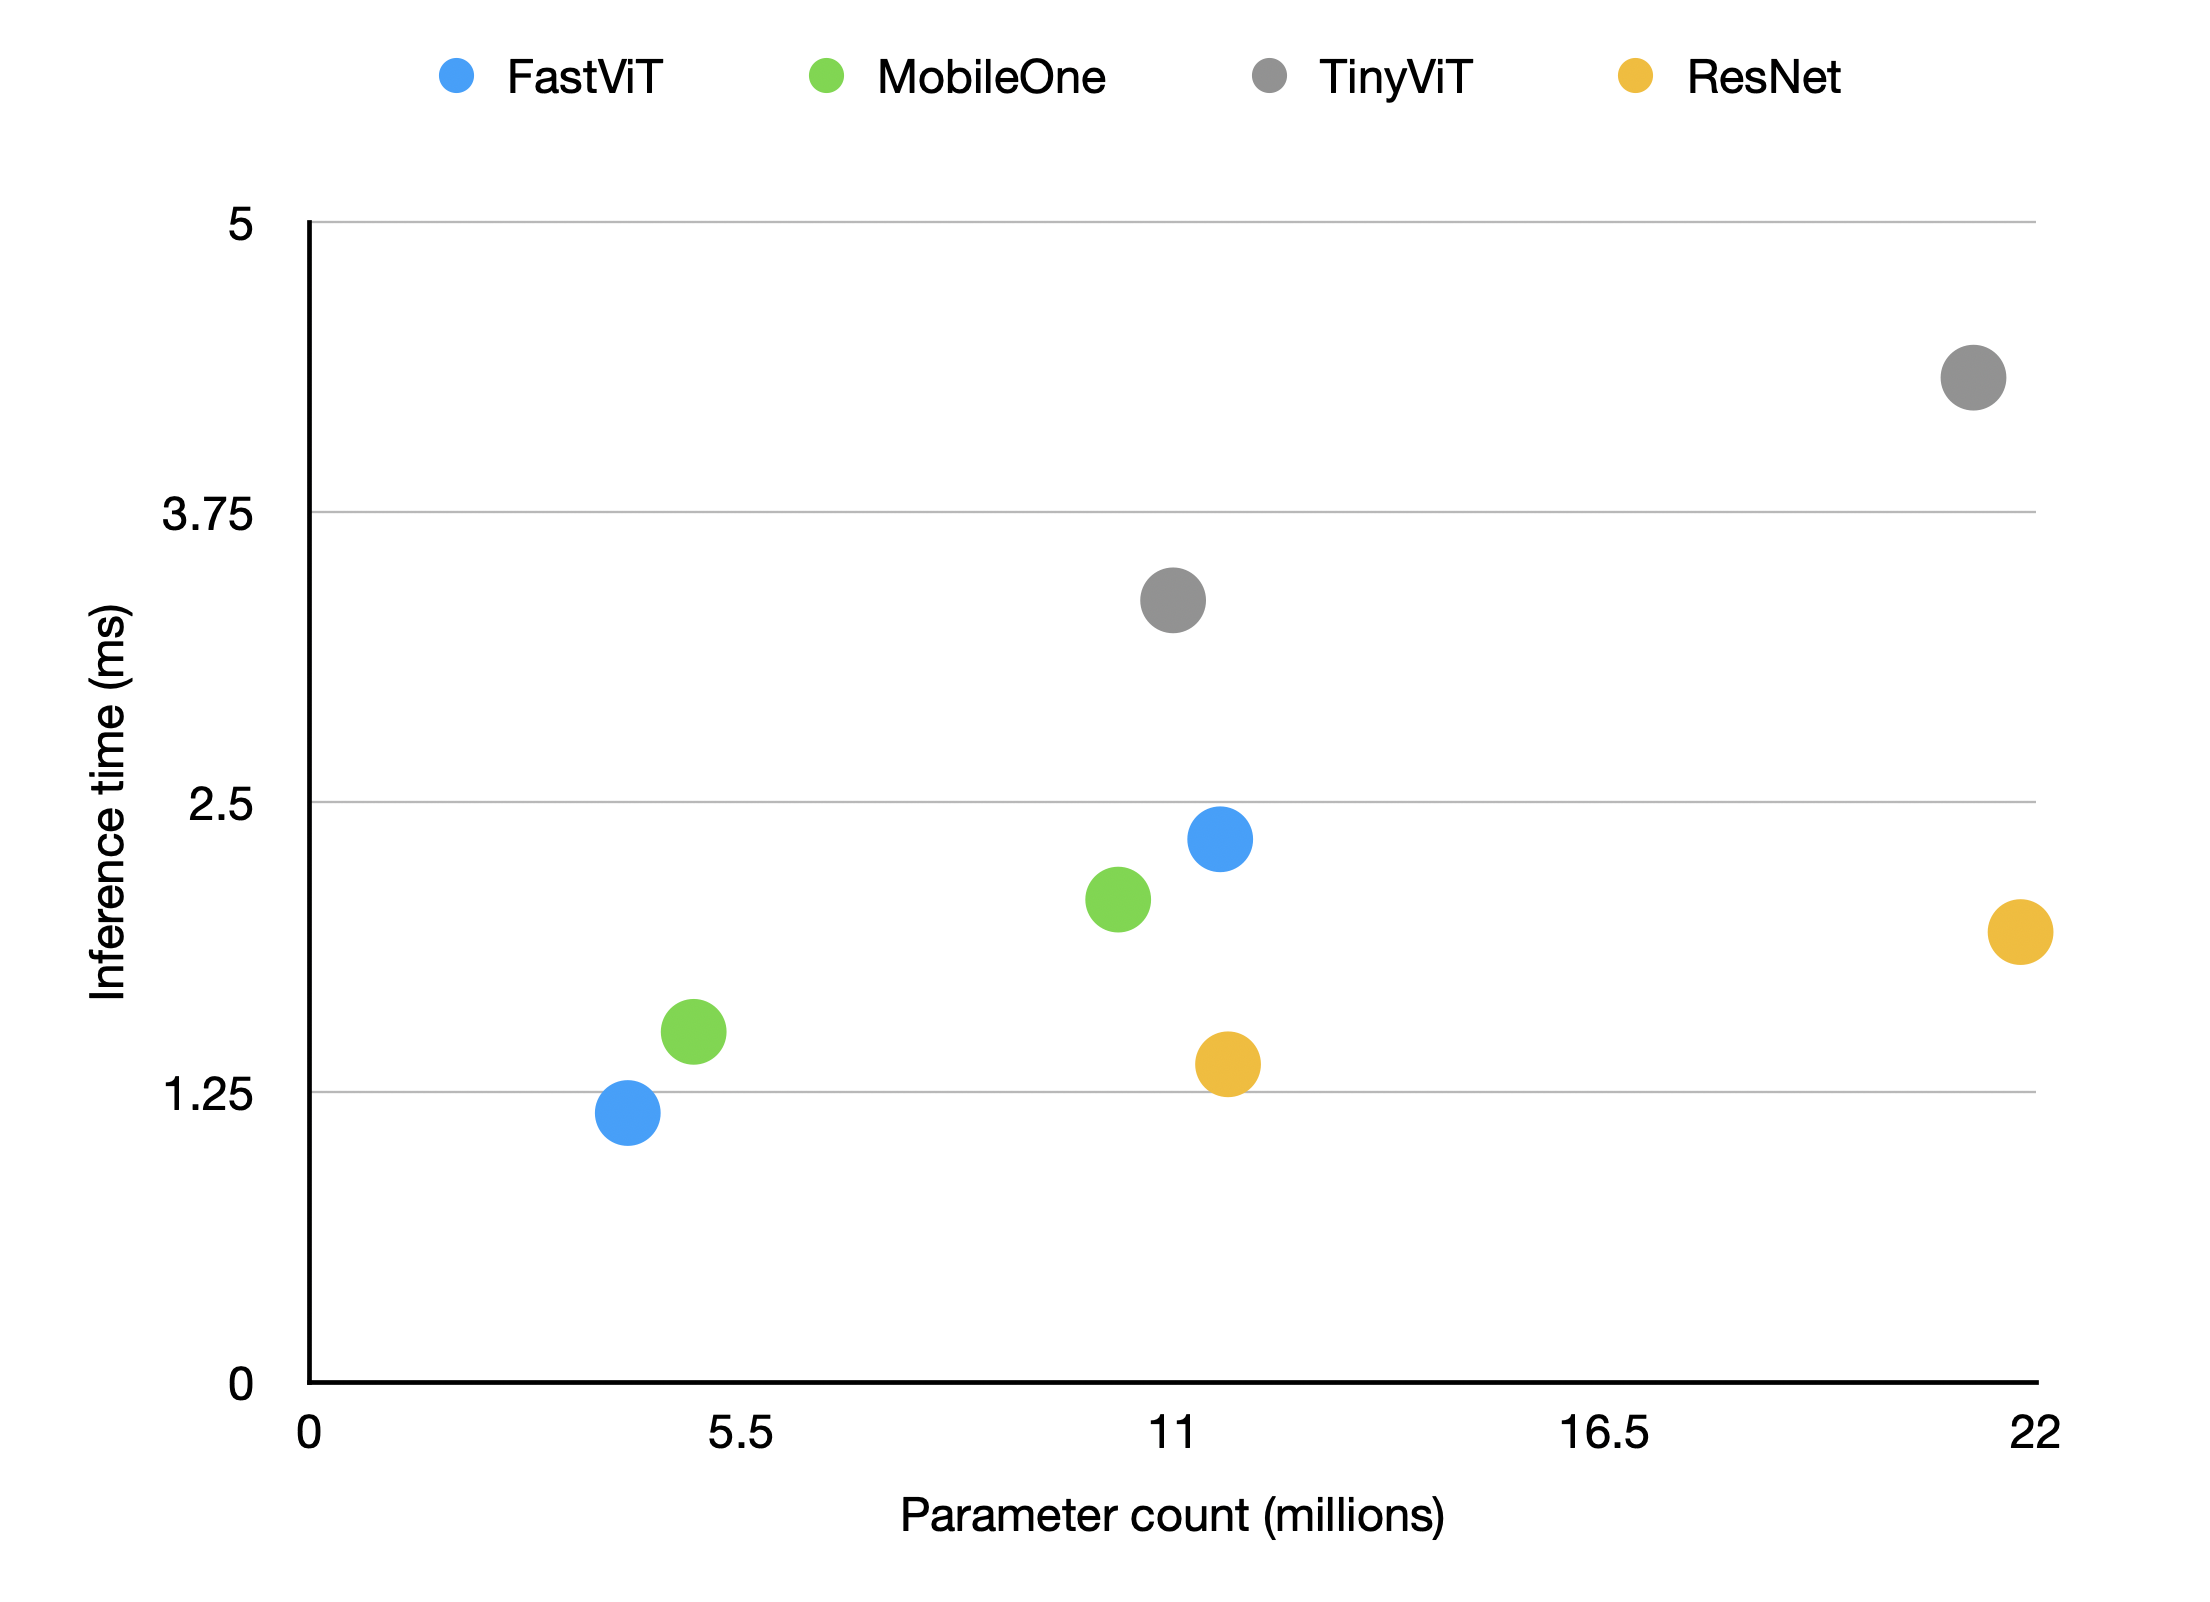
\includegraphics[width=0.8\linewidth]{comparison_latency_inference.png}
    \caption{\label{fig:comparison_latency_inference}Comparison of inference latency versus parameter count for ResNet, TinyViT, MobileOne, and FastViT (both smaller and bigger variants of each model).}
\end{figure}

\subsubsection{Training FastViT}
The experiments with FastViT also illustrate the importance of tailoring training strategies to the model’s initialization. Fine-tuning from pretrained weights required more conservative hyperparameter choices, notably a lower learning rate, to avoid instability in validation performance. Once these adjustments were made, the fine-tuned model not only outperformed the from-scratch training version in accuracy but maintained stable training dynamics. This demonstrates that effective fine-tuning can yield both efficiency and accuracy advantages, provided the training process is calibrated to the pretrained model’s characteristics.

From the confusion matrix, it’s evident that FastViT has difficulties in distinguishing certain classes. For example, classes like ``cat'' and ``dog'', ``ship'' and ``plane'', or ``truck'' and ``car'', often get confused, likely due to similar shapes or textures. This suggest that classes with visually related features or overlapping backgrounds tend to cause more mistakes.

\section{Conclusion}
This section summarizes the primary findings of this study, emphasizing the importance of balancing accuracy and efficiency for mobile deployment, and states which models are best suited under certain constraints. Additionally, recommendations for future work and research is provided based on the review of literature and experimentations made in the project.

\subsection{Main conclusions}

This study provides a comparative analysis of four major neural network architectures—ResNet, TinyViT, MobileOne, and FastViT—under the constraints of on-device mobile deployments. The results underscore the importance of balancing accuracy with practical performance metrics, such as prediction latency and load/compile times. Although certain models, like TinyViT, excelled in top-1 accuracy on ImageNet-1k, their slower prediction speed and higher computational load may limit their viability in latency-critical applications. Conversely, models like FastViT-T8 and MobileOne-S1 offered near-real-time inference speeds on an iPhone 13 Pro at the cost of slightly lower accuracy.

Despite ResNet’s relatively low inference times and minimal operation counts, its top-1 accuracy remains the lowest among the evaluated models. By contrast, MobileOne and FastViT variants—though similar in parameter count to certain ResNet configurations—achieve higher accuracy at the expense of slightly increased inference latencies. This discrepancy can be attributed to the sophisticated reparameterization strategies employed by MobileOne and FastViT, which enable them to pack more representational capacity into a similar-sized parameter space. In other words, while the number of parameters remains comparable, their internal structure is more complex and expressive, ultimately yielding better accuracy even if it requires marginally more time to process on-device.

Among the architectures examined, FastViT stands out as a particularly promising solution for bringing hybrid vision transformers to mobile devices. Traditional ViTs, though effective at modeling global dependencies and achieving high accuracy, are often computationally heavy and memory-intensive, making them challenging to deploy on resource-constrained hardware. FastViT’s hybrid approach, which leverages CNN-like efficiency mechanisms alongside the representational power of transformers, strikes an elegant balance. By employing reparameterization strategies and replacing certain attention layers with large-kernel convolutions, FastViT significantly reduces latency without sacrificing accuracy. This demonstrates that the performance benefits of transformers can indeed be realized within the strict performance budgets of mobile platforms, paving the way for more advanced on-device applications that were previously deemed impractical with conventional ViTs.

From the training perspective, the experiments with FastViT highlight that hyperparameter settings optimized for from-scratch training may not translate directly to fine-tuning scenarios. Adjusting parameters such as learning rates can significantly influence model stability and final performance. By carefully tuning these factors, it is possible to leverage pretrained weights to achieve better generalization and stronger results than from-scratch training on smaller datasets like CIFAR-10.

Looking forward, this work suggests that an ideal mobile deployment strategy should consider both the computational characteristics of the target device and the performance requirements of the application. Models with moderate complexity and thoughtfully adjusted hyperparameters can strike a great balance between accuracy and efficiency.

\subsection{Recommendations for future work}
This subsection offers suggestions for further experiments, involving good practices to load models into an app, training on larger datasets, and model compression.

Xcode’s performance analysis tools provide a detailed window into the model deployment pipeline, enabling practitioners to pinpoint exactly where time is spent during load and compile phases. By examining the operator-level breakdown, developers can identify which parts of the model could be adjusted or pre-optimized. A recommended best practice is to adopt a lazy loading strategy—initialize and load the model once at application start-up or at the user’s first interaction requiring inference, rather than reloading it before every prediction. This approach reduces overhead and ensures that subsequent inferences are executed as rapidly as possible. Additionally, once the model is no longer needed (e.g., the user navigates away from a feature requiring image classification), explicitly unloading it can free up memory and resources, improving the overall responsiveness and efficiency of the application.

Beyond refining the loading and compilation pipeline, exploring model compression techniques offers significant potential to further reduce inference times. A colleague’s suggestion to investigate quantization techniques, which lower numerical precision to shrink model size and speed up inference, stands out as a promising avenue. Similarly, knowledge distillation—transferring knowledge from a larger, more accurate teacher model to a smaller student model—can help preserve accuracy while reducing complexity. For vision transformers, distillation through attention mechanisms provides an elegant means of ensuring that the condensed model retains critical representational capabilities. Such compression strategies, when combined with the deployment and optimization practices outlined above, could yield models that are not only fast and memory-efficient on mobile devices but also competitive in accuracy and robustness.

% References
\newpage
\bibliographystyle{alpha}
\bibliography{sample}

\end{document}